%(BEGIN_QUESTION)
% Copyright 2011, Tony R. Kuphaldt, released under the Creative Commons Attribution License (v 1.0)
% This means you may do almost anything with this work of mine, so long as you give me proper credit

Anta at to radioantenner står på 12-fots tårn, med fri og åpen sikt mellom seg. Hvis driftsfrekvensen er 900 MHz, beregn avstanden mellom tårnene der den første Fresnel-sonen berører bakken mellom antennene. Er denne tårn-til-tårn-avstanden en {\it minimums}- eller {\it maksimums}verdi for praktisk radiodrift?

$$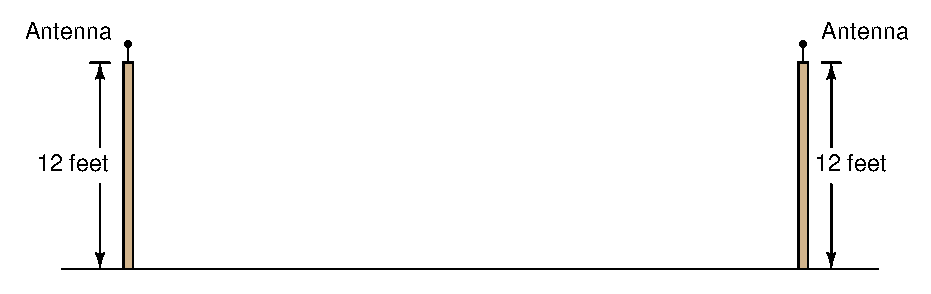
\includegraphics[width=15.5cm]{i00449x01.eps}$$

\vskip 20pt \vbox{\hrule \hbox{\strut \vrule{} {\bf Forslag til sokratisk diskusjon} \vrule} \hrule}

\begin{itemize}
\item{} Identifiser minst én praktisk faktor som vil endre tillatt avstandsverdi mellom de to antennene. Med andre ord: Hva i systemet kan endres slik at en annen avstand blir mulig?
\end{itemize}

\underbar{file i00449}
%(END_QUESTION)





%(BEGIN_ANSWER)

Formelen for å beregne radiusen til Fresnel-sonen er:

$$r = \sqrt{{n \lambda d_1 d_2} \over D}$$

Siden vi er interessert i radiusen i midtpunktet, der $d_1 = d_2 = {D \over 2}$, kan vi sette dette inn i formelen:

$$r = \sqrt{{n \lambda \left({D \over 2}\right)^2} \over D}$$

Forenkling:

$$r = \sqrt{n \lambda {D^2 \over 4} \over D}$$

$$r = \sqrt{n \lambda D^2 \over 4D}$$

$$r = \sqrt{n \lambda D \over 4}$$

Vi finner først bølgelengden ($\lambda$) ved driftsfrekvensen 900 MHz, og løser deretter for avstanden når radiusen til første Fresnel-sone er 12 fot (3.6576 meter):

$$\lambda = {v \over f} = {2.9979 \times 10^{8} \hbox{ m/s} \over 900 \times 10^6 \hbox{ Hz}} = 0.3331 \hbox{ m}$$

$$r = \sqrt{\lambda D \over 4}$$

$$r^2 = {\lambda D \over 4}$$

$$4r^2 = \lambda D$$

$$D = {4r^2 \over \lambda} = {(4) (3.6576 \hbox{ m})^2 \over 0.3331 \hbox{ m}} = 160.65 \hbox{ m}$$

$$\left(160.65 \hbox{ m} \over 1 \right) \left(100 \hbox{ cm} \over 1 \hbox{ m} \right) \left(1 \hbox{ in} \over 2.54 \hbox{ cm} \right) \left(1 \hbox{ ft} \over 12 \hbox{ in} \right) = 527.06 \hbox{ ft}$$

Denne avstanden er en {\it maksimums}verdi, ikke en minimumsverdi. Overskrides 160.65 meter, vil første Fresnel-sone berøre bakken midt mellom antennene.

%(END_ANSWER)





%(BEGIN_NOTES)






\vfil \eject

\noindent
{\bf Oppsummeringsquiz:}

Når frekvensen til et radiosignal økes:

\begin{itemize}
\item{} Øker dempningen i banen, og Fresnel-sonen blir smalere
\vskip 5pt
\item{} Øker dempningen i banen, og Fresnel-sonen blir bredere
\vskip 5pt
\item{} Er banedempningen uendret, og Fresnel-sonen blir smalere
\vskip 5pt
\item{} Minker banedempningen, og Fresnel-sonen blir smalere
\vskip 5pt
\item{} Minker banedempningen, og Fresnel-sonen blir bredere
\vskip 5pt
\item{} Øker banedempningen, og Fresnel-sonen er uendret
\end{itemize}


%INDEX% Electronics review, Fresnel zones for radio links

%(END_NOTES)
